\def\figpath{tex/2_LC-Oszillator/pictures}
\graphicspath{{tex/2_LC-Oszillator/pictures/}}

\chapter{LC-Oszillator}
Das 2. Kapitel behandelt die Analyse der in Abb. \ref{fig_Kap2_01:Oszillator} gezeigten Oszillatorschaltung.

\begin{figure}[H]
    \centering
    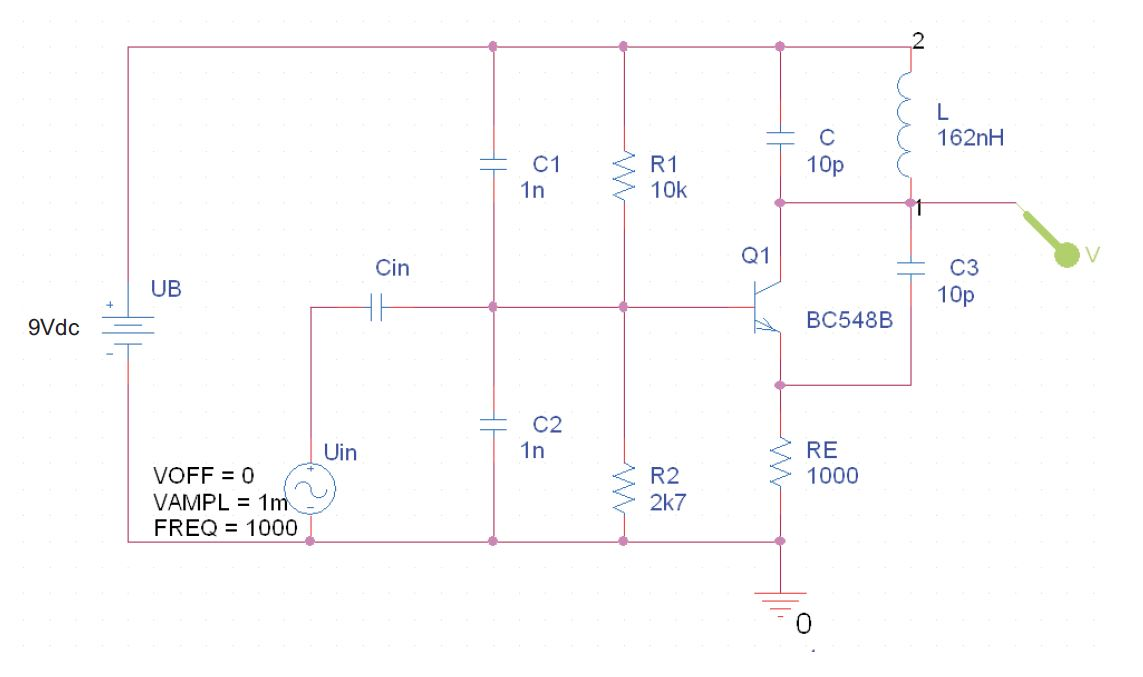
\includegraphics[width = \textwidth]{\figpath/Oszillatorschaltung.jpg}
    \caption{Oszillatorschaltung}
    \label{fig_Kap2_01:Oszillator}
\end{figure}

\section{Schwingbedingung}
Zuerst soll auf Basis des Kleinsignalersatzschaltbildes die Resonanzfrequenz berechnet werden. Hierbei dürfen lt. Praktikumsskript die Kapazitäten $C_1$ und $C_2$ als unendlich angenommen werden. Außerdem sind die parasitären Kapazitäten des Transistors lt. Abb. \ref{fig_Kap2_02:parasit} zu berücksichtigen.

\begin{figure}[H]
    \centering
    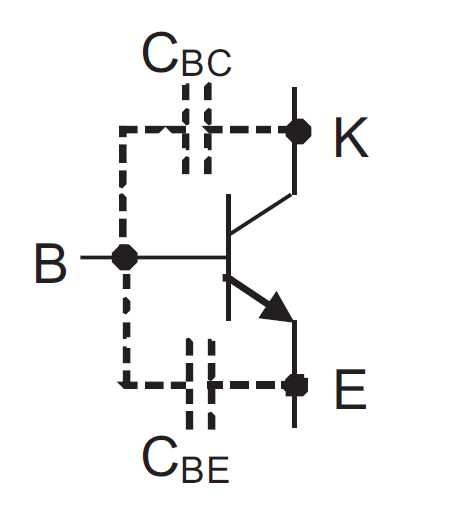
\includegraphics[width = 0.3\textwidth]{\figpath/parasit.jpg}
    \caption{Oszillatorschaltung}
    \label{fig_Kap2_02:parasit}
\end{figure}

Das KSESB der Oszillatorschaltung sieht folgendermaßen aus:

\begin{figure}[H]
	\centering
	\def\svgwidth{0.8\textwidth}
	\input{\figpath/KSESB.pdf_tex}
	\caption{KSESB der Oszillatorschaltung} 
	\label{fig:01_QStatAufbau} 
\end{figure}

Fasst man die relevanten Bauteile zu zwei Ersatzimpendazen

\begin{equation}
    \underline{Z}_1 = \frac{1}{\underline{Y}_1} = \frac{1}{\frac{S}{B}+\frac{1}{R_E}+j  \omega C_{BE}}
\end{equation}

\begin{equation}
    \underline{Z}_2 = \frac{1}{\underline{Y}_2} = \frac{1}{\frac{1}{j\omega L}+j \omega \left( C_{BC} + C \right)}
\end{equation}

zusammen, so lässt sich die Schaltung vereinfacht darstellen:

\begin{figure}[H]
	\centering
	\def\svgwidth{0.6\textwidth}
	\input{\figpath/KSESB2.pdf_tex}
	\caption{Vereinfachtes KSESB der Oszillatorschaltung} 
	\label{fig:01_QStatAufbau} 
\end{figure}

Laut der Kirchhoffschen Maschenregel kann nun folgender Ausdruck gebildet werden:

\begin{equation}
    u_{BE} \cdot \left( 1 + \frac{S + \underline{Y}_1}{j \omega C_3} + \frac{\underline{Y}_1}{\underline{Y}_2} \right) = 0
\end{equation}

Setzt man nun die Ausdrücke der Ersatzadmittanzen ein folgt:
\begin{equation}
    u_{BE} \cdot \left( 1 + \frac{S + \frac{S}{B}+\frac{1}{R_E}+j  \omega C_{BE}}{j \omega C_3} + \frac{\frac{S}{B}+\frac{1}{R_E}+j  \omega C_{BE}}{\frac{1}{j\omega L}+j \omega \left( C_{BC} + C \right)} \right) = 0
\end{equation}

Die Steuergröße des Oszillators, die Basis-Emitterspannung $u_{BE}$, darf naturgemäß nicht verschwinden, womit sich die Schwingbedingung im komplexen Zahlenraum ergibt:

\begin{equation}
    1 + \frac{S + \frac{S}{B}+\frac{1}{R_E}+j  \omega C_{BE}}{j \omega C_3} + \frac{\frac{S}{B}+\frac{1}{R_E}+j  \omega C_{BE}}{\frac{1}{j\omega L}+j \omega \left( C_{BC} + C \right)} = 0
\end{equation}

Betrachtet man nun den Real- und Imaginärteil obiger Gleichung einzeln, erhält man 2 reelle Schwingbedingungen, was mithilfe des Computeralgebraprogramms \textit{MAXIMA} hergeleitet wurde.\\
Für den Realteil gilt:

\begin{equation}
\label{glng_01}
    1 + \frac{C_{BE}\omega}{\omega (C_{BC} + C) - \frac{1}{\omega L}} + \frac{C_{BE}}{C_3} = 0
\end{equation}

Für den Imaginärteil ergibt sich folgende Gleichung:
\begin{equation}
    \label{glng_03}
    -\frac{\frac{S}{B}+\frac{1}{R_E}}{\omega(C_{BC} + C)-\frac{1}{\omega L}} - \frac{S\left(\frac{1}{B} + 1\right) + \frac{1}{R_E}}{\omega C_3} = 0
\end{equation}

Der variable Emitterwiderstand $R_E$ kommt in Gleichung \ref{glng_01} nicht vor, wodurch sich ein Ausdruck für die Resonanzkreisfrequenz aus einer quadratischen Gleichung finden lässt, wobei natürlich die negative Lösung verworfen wird: 

\begin{equation}
    \label{glng_02}
    \omega = \sqrt{\frac{C_{BE} + C_3}{\left( \left( C_{BC} + C_3 + C\right)C_{BE} + C_3 C_{BC} + CC_3 \right) L}}
\end{equation}

Setzt man nun die Lösung \ref{glng_02} in Glng. \ref{glng_03} ein, lässt sich ein Ausdruck für den variablen Widerstand $R_E$ in Abhängigkeit der Steilheit $S$ des Transistors im jeweiligen Arbeitspunkt finden:

\begin{equation}
    R_E = \frac{B \cdot C_3}{S \cdot \left( B C_{BE} - C_3\right)}
\end{equation}

\section{Simulation}